\section{Non-convex problems}
\sectionlabel{non_convexity}

This lecture provides the important information on how non-convex problems differ from convex problems. The major issue in non-convex problems is that it can be difficult to find the global minimum because algorithms can easily get stuck in the possibly numerous local minima and saddle points.

\begin{center}
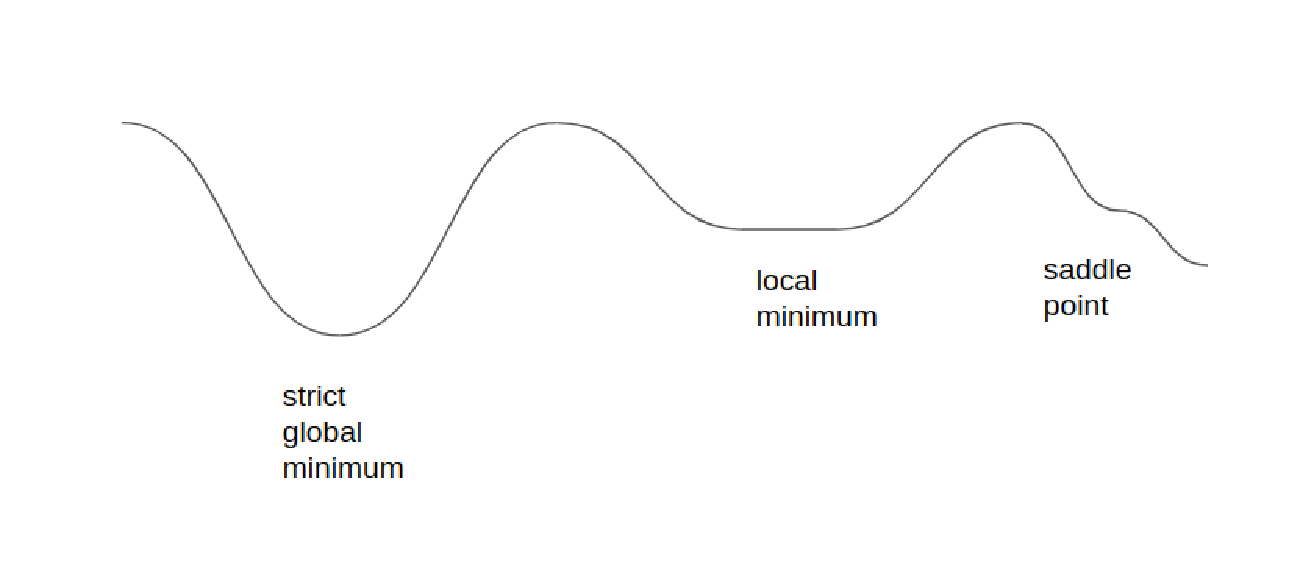
\includegraphics[width=1.0\linewidth, height=0.4\linewidth]{figures/lecture_17_non_convex_graph.pdf} 
\end{center}

\subsection{Local minima}

\begin{definition}[Local minimum]
A point $x^*$ is an unconstrained \textit{local minimum} if there exist $\epsilon > 0$ such that $f(x^*) \le f(x)$ for all $x$ with $\|x - x^*\| < \epsilon$.
\end{definition}

\begin{definition}[Global minimum]
A point $x^*$ is an unconstrained \textit{global minimum} if $f(x^*) \le f(x)$ for all $x$.
\end{definition}

For both definitions, we say ''strict'' if these inequalities are strict.

\begin{proposition}[Necessary Conditions for local minimum]
\propositionlabel{nc for local min}
Let $x^*$ be an unconstrained local minimum of $f\colon \R^n \to\R$ and assume $f$ is continuously differentiable ($C^1$) in an open set containing $x^*$. Then
\begin{enumerate}
    \item $\nabla f(x^*) = 0$ (First-Order Necessary Condition)
    \item If in addition $f$ is twice continuously differentiable in an open set around $x^*$, then $\nabla^2f(x^*) \succeq 0$. (Second Order Necessary Condition)
\end{enumerate}
\end{proposition}

\begin{proof}[Proof of \propositionref{nc for local min}.]
Fix any direction $d \in \R^n$.
\begin{enumerate}
    \item $g(\alpha) := f(x^* + \alpha d)$. Then
    \begin{align}
        0 &\le \lim_{\alpha \to 0} \frac{f(x^* + \alpha d) - f(x^*)}{\alpha} \label{eqn:0}\\
        &= \frac{\partial g(0)}{\partial \alpha} \nonumber\\
        &= d^\trans \nabla f(x^*) \nonumber
    \end{align}
    Inequality \ref{eqn:0} follows because $x^*$ is a local minimum, $0 \le f(x^* + \alpha d) - f(x^*)$ for sufficiently small alpha. So, we can construct a sequence with only positive $\alpha$ that converges to $x^*$ such that each element $0 \le \frac{f(x^* + \alpha_n d) - f(x^*)}{\alpha_n}$ which implies that statement given that $f$ is locally differentiable.\\
    \newline
    Since $d$ is arbitrary, this implies that $\nabla f(x^*) = 0$.
    \item First we represent $f(x^* + \alpha d) - f(x^*)$ using the 2nd order Taylor expansion.
    \begin{align*}
        f(x^* + \alpha d) - f(x^*) &= \alpha \nabla f(x^*)^\trans d + \frac{\alpha^2}{2}d^\trans \nabla^2 f(x^*)d + O(\alpha^2) \nonumber\\
        &= \frac{\alpha^2}{2} d^\trans \nabla^2 f(x^*) d + O(\alpha^2)\\
    \end{align*}
    Now we do the following
    \begin{align*}
        0 &\le \lim_{\alpha \to 0} \frac{f(x^* + \alpha d) - f(x^*)}{\alpha^2}\\
        &= \lim_{\alpha \to 0} \frac{1}{2}d^\trans \nabla^2 f(x^*) d + \frac{O(\alpha^2)}{\alpha^2}\\
        &= \frac{1}{2}d^\trans \nabla^2 f(x^*) d
    \end{align*}
    Because $d$ is arbitrary, this implies that $\nabla^2 f(x^*) \succeq 0$ (Positive semidefinite).
    
\end{enumerate}
\end{proof}

Note that $\nabla f(x^*) = 0$ alone does not imply $x^*$ is a local minimum. Even the necessary conditions $\nabla f(x^*) = 0$ and $\nabla^2 f(x^*) \succeq 0$ does not imply $x^*$ is a local minimum. This is because it could be that $\nabla^2 f(x^*) = 0$, but the 3rd order is not 0. For example in the 1d case, $x^* = 0$ for $f(x) = x^3$ satisfies these conditions, but is not a local minimum. Now, we will look at the actual sufficient conditions for a local minimum, but these conditions can only detect strict local minima.

\begin{proposition}[Sufficient conditions for strict local minimum]
\propositionlabel{sufficient condition for strict local min}
    Let $f\colon \R^n \to \R$ be twice continuously differentiable ($C^2$) over an open set $S$. Suppose $x \in S$ such that $\nabla f(x^*) = 0$ and $\nabla^2f(x) \succ 0$ (positive definite). Then, $x^*$ is a strict unconstrained local minimum.
\end{proposition}

\begin{proof}[Proof of \propositionref{sufficient condition for strict local min}.]
Fix $d \in \R^n$. Note that $d^\trans \nabla^2 f(x^*) d \ge \lambda_{\text{min}} \|d\|^2$, where $\lambda_\text{min}$ is the smallest eigenvalue of $\nabla^2 f(x^*)$.
\begin{align}
    f(x^* + d) - f(x^*) &= \nabla f(x^*)^\trans d + \frac{1}{2}d^\trans \nabla^2 f(x^*)d + O(\|d\|^2) \label{eqn:1}\\
    &\ge \frac{\lambda_{\text{min}}}{2} \|d\|^2 + O(\|d\|^2) \nonumber\\
    &= (\frac{\lambda_{\text{min}}}{2} + \frac{O(\|d\|^2)}{\|d\|^2}) \|d\|^2 \nonumber\\
    &> 0 \label{eqn:2}
\end{align}
Equality \ref{eqn:1} follows from using the 2nd Order Taylor expansion.\\
Inequality \ref{eqn:2} follows for sufficiently small $\|d\|$.\\ 
\newline
Therefore, $x^*$ must be a strict local minimum.
\end{proof}

\subsection{Stationary points}

For non-convex problems we must accept that gradient descent cannot always find the global minimum, but can it at least find a nearby local minimum? It turns out that for many problems we care about it can usually, but not always!

\begin{definition}[Stationary point]
We say a point $x \in \R^n$ is a stationary point of $f\colon \R^n \to \R$ if $\nabla f(x) = 0$.
\end{definition}

\begin{proposition}
\propositionlabel{gd converges}
Gradient Descent converges to a stationary point.
\end{proposition}

\begin{proof}[Proof of \propositionref{gd converges}]
Suppose $x' = x - \eta \nabla f(x)$. From Taylor expansion we get the following
\begin{align}
    f(x') &= f(x) + \nabla f(x)^\trans (x' - x) + O(\|x' - x\|) \nonumber\\
    &= f(x) - \eta\|\nabla f(x)\|^2 + O(\eta \|\nabla f(x)\|) \nonumber\\
    &= f(x) - \eta \|\nabla f(x)\|^2 + O(\eta) \label{eqn:3}
\end{align}
Equality \ref{eqn:3} is justified because we control $\eta$, and $\|\nabla f(x)\|$ is a constant with respect to $\eta$.\\
\newline
Now we need to worry about selecting step sizes.
\subsubsection{Minimization Rule / Line Search}
Given a descent direction $d$ (example $d = - \nabla f(x)$), let our step rate $\eta$ be as follows
\[
    \eta \in \argmin_{\eta \ge 0} f(x + \eta d)
\]

Using this procedure is called \textbf{Line Search} because we search for the best step size along the direction $d$. However, exact line search can be expensive due to the argmin.\\
\newline
Instead, we can approximate this minimization by using the \textbf{Armijo Rule}. 
Fix 
\[
    \gamma, s, \sigma < 1
\]
Put $\eta = \gamma^m s$ where $m$ is the smallest non-negative integer such that
\[
    f(x) - f(x + \gamma^m s d) \ge - \sigma \gamma^m s \nabla f(x)^\trans d
\]
Think of $s$ as an initial learning rate. If $s$ causes sufficient decrease then stop, otherwise keep multiplying by $\gamma$ until you do. Typical choices for parameters are 
\[
    \gamma = \frac{1}{2}, \sigma = \frac{1}{100}, s = 1
\]
\newline
Notice that as long as $d$ satisfies $-\nabla f(x)^Td > 0$ that the inequality ensures that our function sequence will decrease.

\begin{proposition}
\propositionlabel{converge to stationary point}
Assume that $f$ if continuous and differentiable ($C^1$), and let $\{x_t\}$ be a sequence generated by $x_{t+1} = x_t - \eta_t \nabla f(x_t)$ where $\eta_t$ is selected by the Armijo rule. Then, every limit point of $\{x_t\}$ is a stationary point.
\end{proposition}

\begin{proof}[Proof of \propositionref{converge to stationary point}]
Let $\bar{x}$ be a limit point. By continuity $\{f(x_t)\}$ converges to $f(\bar{x})$ and therefore:
\[
    f(x_t) - f(x_{t+1}) \to 0
\]
By definition of Armijo rule:
\begin{equation}
    f(x_t) - f(x_{t+1}) \ge -\sigma \eta_t \|\nabla f(x_t)\|^2 \label{eqn:4}
\end{equation}
Suppose for the sake of contradiction that $\bar{x}$ is not a stationary point of $f$. Then,
\[
    \limsup_{t \to \infty} -\|\nabla f(x_t)\|^2 < 0
\]
By inequality \ref{eqn:4}, this must mean that $\eta_t \to 0$. This implies $\exists t_0$ such that $\forall t \ge t_0$
\[
    f(x_t) - f(x_t - \frac{\eta_t}{\gamma} \nabla f(x_t)) < \frac{\sigma \eta_t}{\gamma} \|\nabla f(x_t)\|^2
\]
Because $\eta_t \to 0$, we know that after some $t_0$ all step sizes are chosen with a $m\ge 1$. Therefore, going back one iteration of Armijo rule was not good enough to satisfy the inequality or else some previous step size would have been chosen.\\
\newline
Now let $\tilde{\eta_t} = \frac{\eta_t}{\gamma}$ and we can continue as follows
\begin{align}
    \frac{f(x_t) - f(x_t - \tilde{\eta_t} \nabla f(x_t))}{\tilde{\eta_t}} &< \sigma \|\nabla f(x)\|^2 &\Rightarrow \nonumber\\
    \nabla f(x_t - \tilde{\eta_t} \nabla f(x_t))^T \nabla f(x_t) &< \sigma \|\nabla f(x)\|^2 &\Rightarrow \label{eqn:5}\\
    \|\nabla f(x_t) \|^2 &\le \sigma \|\nabla f(x_t) \|^2 & \label{eqn:6}
\end{align}
\newline
Inequality \ref{eqn:5} follows from using Mean Value Theorem (MVT)\\
Inequality \ref{eqn:6} follows by taking the limit as $\eta_t \to 0 \Rightarrow \tilde{\eta_t} \to 0$\\
\newline
This is a contradiction because $0 < \sigma < 1$. Therefore, the limit point $\bar{x}$ is a stationary point of $f$.
\end{proof}
Therefore, if we can use the Armijo rule to determine step sizes that guarantee that gradient descent will converge to a stationary point.
\end{proof}

\subsection{Saddle points}

Now that we have found that gradient descent will converge to a stationary point, how concerned should we be that the stationary point is not a local minimum?

\begin{definition}[Saddle points]
Saddle points are stationary points that are not local optima.
\end{definition}
This means that if $f$ is twice differentiable then $\nabla^2 f(x)$ has both positive and negative eigenvalues.
\subsubsection{How do saddle points arise?}
In most non-convex problems there exists several local minima. This is clear to see in problems that have natural symmetry such as in a two layer fully connected neural networks. 
\begin{center}
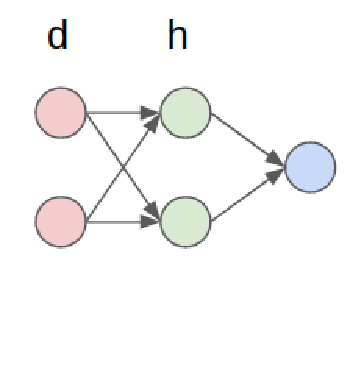
\includegraphics[width=0.3\linewidth, height=0.3\linewidth]{figures/lecture_17_neural_network.pdf} 
\end{center}
Notice that any permutation of the units of the hidden layer would preserve the same function, so we have at least $h!$ local minima. Typically a convex combination of two distinct local minima in a non-convex problem is not a local minimum. In the case where $\nabla f(x)$ is differentiable, then by Mean Value Theorem we know that there must exist another stationary point between any two local minima. So, there often exists at least one saddle point between any two distinct local minima. Hence, many local minima tends to lead to many saddle points.\\
\newline
However, recent work has demonstrated that saddle points are usually not a problem.
\begin{enumerate}
    \item Gradient descent does not converge to strict saddle points from a random initialization. \cite{DBLP:journals/corr/GeHJY15}
    \item Saddle points can be avoided with noise addition. \cite{DBLP:journals/corr/abs-1710-07406}
\end{enumerate}
